\documentclass[9pt,aspectratio=169]{beamer}

% ============================================================
% PACKAGES
% ============================================================
\usepackage[utf8]{inputenc}
\usepackage[T1]{fontenc}
\usepackage{amsmath,amssymb}
\usepackage{graphicx}
\usepackage[table]{xcolor}
\usepackage{booktabs}
\usepackage{multirow}
\usepackage{array}
\usepackage{hyperref}
\usepackage{lmodern}
\usepackage{tikz}
\usetikzlibrary{positioning,arrows.meta,calc,shapes.multipart}

% ============================================================
% THEME
% ============================================================
\usetheme{Madrid}
\usecolortheme{seahorse}
\setbeamertemplate{navigation symbols}{}
\setbeamertemplate{footline}{%
  \leavevmode%
  \hbox{%
    \begin{beamercolorbox}[wd=.5\paperwidth,ht=2.25ex,dp=1ex,left,leftskip=1em]{author in head/foot}%
      \usebeamerfont{author in head/foot}\insertshortauthor\ |\ \insertshortinstitute
    \end{beamercolorbox}%
    \begin{beamercolorbox}[wd=.4\paperwidth,ht=2.25ex,dp=1ex,center]{title in head/foot}%
      \usebeamerfont{title in head/foot}\insertshorttitle
    \end{beamercolorbox}%
    \begin{beamercolorbox}[wd=.1\paperwidth,ht=2.25ex,dp=1ex,right,rightskip=1em]{date in head/foot}%
      \usebeamerfont{date in head/foot}\insertframenumber/\inserttotalframenumber
    \end{beamercolorbox}}%
}
\setbeamerfont{frametitle}{size=\small,series=\bfseries}
\setbeamerfont{title}{size=\large,series=\bfseries}
\setbeamerfont{subtitle}{size=\footnotesize}
\setbeamerfont{block title}{size=\footnotesize,series=\bfseries}
\setbeamerfont{block body}{size=\footnotesize}
\setbeamertemplate{itemize items}[circle]
\setbeamertemplate{enumerate items}[default]

\setlength{\leftmargini}{1.1em}
\setlength{\leftmarginii}{0.9em}
\setlength{\itemsep}{0pt}
\setlength{\parskip}{0pt}

% ============================================================
% COLOURS
% ============================================================
\definecolor{darkred}{RGB}{150,20,20}
\definecolor{steelblue}{RGB}{50,90,160}
\definecolor{forestgreen}{RGB}{30,110,50}
\definecolor{amberc}{RGB}{200,140,20}

% ============================================================
% TITLE PAGE
% ============================================================
\title[Banking Credit Risk Platform]{%
  Banking Credit Risk Calculator:\\[2pt]
  A Basel III Compliant, ML-Powered Credit Risk Platform}

\subtitle{PD Modelling · Policy Governance · RM Decision Support · Regulatory \& Financial Reporting}

\author[Credit Risk Engineering]{Credit Risk \& Banking Intelligence Platform}

\institute[Axis Bank]{%
  Banking Credit Risk Calculator --- Internal Solution Overview}

\date{July 2026}

% ============================================================
\begin{document}
% ============================================================

% SLIDE — TITLE
\begin{frame}
  \titlepage
\end{frame}

% SLIDE — OUTLINE
\begin{frame}{Outline}
  \tableofcontents
\end{frame}

% ===========================================================
\section{Platform Overview}
% ===========================================================

% SLIDE — EXECUTIVE SUMMARY
\begin{frame}{Executive Summary}
\vspace{-2pt}
\begin{block}{What this platform is}
  \footnotesize
  A single Flask-based application that takes a bank from \textbf{raw borrower data} to a
  \textbf{governed credit decision} to \textbf{regulator-ready reporting} --- covering
  origination, ML risk scoring, deterministic policy, human-in-the-loop approval,
  Basel III capital/liquidity reporting, and financial statements, for one global banking group.
\end{block}
\vspace{5pt}
\begin{columns}[T]
  \column{0.55\textwidth}
    \textbf{Why it matters}
    \begin{itemize}\setlength\itemsep{3pt}
      \item[\small$\bullet$] Replaces spreadsheet-based, disconnected credit assessment with a
            single traceable pipeline: model $\to$ policy $\to$ human decision $\to$ report
      \item[\small$\bullet$] Every recommendation is \textbf{explainable} (SHAP-driven attribution)
            and every RM decision is \textbf{hash-chained} for audit
      \item[\small$\bullet$] Basel III capital/liquidity ratios and financial statements are
            derived from the \textbf{same underlying loan ledger} --- not reconciled separately
    \end{itemize}
  \column{0.42\textwidth}
    \begin{block}{Scale (grounded ledger)}
      \footnotesize
      \begin{itemize}\setlength\itemsep{2pt}
        \item 9 real-world banks across 6 countries (India, USA, UK, Singapore, UAE, Australia)
        \item Group $\to$ Region $\to$ Country $\to$ Bank hierarchy
        \item All capital/liquidity/NPA/P\&L figures roll up from per-loan records
      \end{itemize}
    \end{block}
\end{columns}
\end{frame}

% SLIDE — SIX DEPARTMENTS
\begin{frame}{Six Departments, One Platform}
\vspace{-2pt}
\begin{center}
\footnotesize
\setlength{\tabcolsep}{5pt}
\begin{tabular}{lp{7.6cm}l}
  \toprule
  \textbf{Department} & \textbf{What it does} & \textbf{Route}\\
  \midrule
  Credit Risk            & ML PD, LGD, RWA, EL, pricing --- single-borrower calculator     & \texttt{/}\\
  Banking Operations     & Multi-bank dashboards, customer/account/loan ledger              & \texttt{/operations/}\\
  Regulatory Reporting   & Basel III/RBI capital (CRAR, LCR, NSFR) per bank \& client        & \texttt{/regulatory/}\\
  Relationship Mgmt      & Machine recommendation $\to$ RM accept/reject $\to$ PDF report    & \texttt{/relationship/}\\
  Financial Reporting    & Balance sheet, P\&L, key ratios, Pillar 3 --- any roll-up scope   & \texttt{/financials/}\\
  Global Reference Data  & Countries, macro indicators, sovereign ratings                    & \texttt{/reference/}\\
  \bottomrule
\end{tabular}
\end{center}
\vspace{6pt}
\begin{alertblock}{One origination channel, six consuming views}
  \footnotesize
  A borrower is captured \textbf{once} on the Credit Risk calculator. Every other department
  (Operations, Regulatory, RM, Financials) reads from the same ledger --- there is no
  duplicate data entry and no reconciliation step between departments.
\end{alertblock}
\end{frame}

% SLIDE — ARCHITECTURE
\begin{frame}{Architecture \& Technology Stack}
\vspace{-2pt}
\begin{columns}[T]
  \column{0.46\textwidth}
    \footnotesize
    \begin{tabular}{ll}
      \toprule
      \textbf{Layer} & \textbf{Technology}\\
      \midrule
      Web server  & Flask 3.x + gunicorn\\
      ML model    & XGBoost --- 4 segment models\\
      Scheduler   & APScheduler (background)\\
      Database    & SQLite \texttt{bank.db} (raw SQL)\\
      Frontend    & Vanilla HTML5 / CSS3 / JS\\
      Deployment  & GCP App Engine (Py 3.10)\\
      \bottomrule
    \end{tabular}
    \vspace{6pt}

    \textbf{Key backend modules}
    \begin{itemize}\setlength\itemsep{1pt}
      \footnotesize
      \item[\small$\bullet$] \texttt{assessment\_engine.py} --- full borrower findings
      \item[\small$\bullet$] \texttt{policy\_engine.py} --- deterministic rules
      \item[\small$\bullet$] \texttt{decision\_orchestrator.py} --- Machine Recommendation
      \item[\small$\bullet$] \texttt{shap\_explainer.py} --- feature attribution
      \item[\small$\bullet$] \texttt{regulatory\_engine.py} --- Basel III / RBI
      \item[\small$\bullet$] \texttt{alm\_engine.py} --- asset-liability management
    \end{itemize}

  \column{0.50\textwidth}
    \begin{center}
    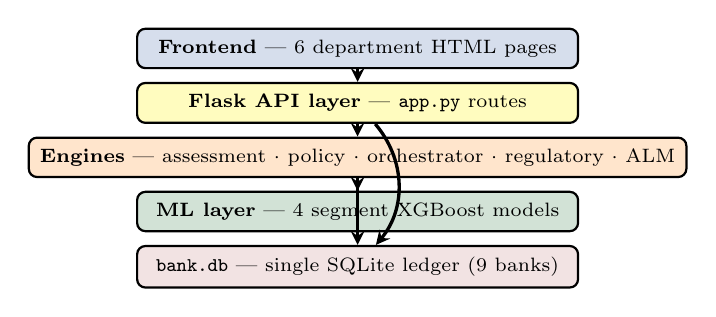
\begin{tikzpicture}[
        mbox/.style={draw, rounded corners=3pt, align=center, minimum width=5.6cm,
                     inner sep=4pt, font=\scriptsize, thick},
        arr/.style={->, very thick, >=stealth}
    ]
    \node[mbox, fill=steelblue!20] (ui) at (0,0) {\textbf{Frontend} --- 6 department HTML pages};
    \node[mbox, fill=yellow!25, below=0.16cm of ui] (api) {\textbf{Flask API layer} --- \texttt{app.py} routes};
    \node[mbox, fill=orange!20, below=0.16cm of api] (eng) {\textbf{Engines} --- assessment $\cdot$ policy $\cdot$ orchestrator $\cdot$ regulatory $\cdot$ ALM};
    \node[mbox, fill=forestgreen!20, below=0.16cm of eng] (ml) {\textbf{ML layer} --- 4 segment XGBoost models};
    \node[mbox, fill=darkred!12, below=0.16cm of ml] (db) {\textbf{\texttt{bank.db}} --- single SQLite ledger (9 banks)};
    \draw[arr] (ui) -- (api);
    \draw[arr] (api) -- (eng);
    \draw[arr] (eng) -- (ml);
    \draw[arr] (eng) -- (db);
    \draw[arr] (api) to[bend left=40] (db);
    \end{tikzpicture}
    \end{center}
\end{columns}
\end{frame}

% ===========================================================
\section{ML Credit Risk Engine}
% ===========================================================

% SLIDE — PD MODEL
\begin{frame}{Probability of Default (PD) --- Segment-Specific XGBoost}
\vspace{-2pt}
{\footnotesize A single aggregate model under-serves heterogeneous portfolios --- a Corporate
borrower and a Retail-Mortgage borrower default for different reasons. The platform trains
\textbf{one XGBoost classifier per Basel exposure class}, each promoted independently.}\\[6pt]
\begin{center}
\footnotesize
\begin{tabular}{lrrrl}
  \toprule
  \textbf{Exposure Class} & \textbf{AUC-ROC} & \textbf{Accuracy} & \textbf{Recall} & \textbf{SA Risk Weight}\\
  \midrule
  CORPORATE          & 0.754 & 60.9\% & 73.6\% & 100\%\\
  SME                & 0.764 & 63.7\% & 79.4\% & 85\%\\
  RETAIL\_MORTGAGES  & 0.758 & 63.0\% & 76.5\% & 35\%\\
  RETAIL\_OTHER      & 0.753 & 65.4\% & 78.8\% & 75\%\\
  \bottomrule
\end{tabular}
\end{center}
\vspace{6pt}
\begin{columns}[T]
  \column{0.55\textwidth}
    \textbf{Feature schema (36 inputs)}
    \begin{itemize}\setlength\itemsep{2pt}
      \item[\small$\bullet$] Core financial ratios: \texttt{de\_ratio}, \texttt{interest\_coverage},
            \texttt{profitability}, \texttt{liquidity\_ratio}
      \item[\small$\bullet$] 15 borrower / bureau attributes (age, income, CIBIL, FOIR, employment,
            delinquency history)
      \item[\small$\bullet$] 4 country macro indicators + 8 trend / regime-shift features
            (period-over-period deltas + a composite macro distress score)
      \item[\small$\bullet$] 5 ``other-circumstances'' behavioural signals (ECS/NACH bounces,
            other-lender exposure, income disruption, sector stress, LTV drift)
    \end{itemize}
  \column{0.42\textwidth}
    \textbf{Governance}
    \begin{itemize}\setlength\itemsep{2pt}
      \item[\small$\bullet$] \texttt{model\_feature\_frame()} aligns any partial input to the
            full schema (neutral defaults for missing fields)
      \item[\small$\bullet$] Promotion requires R\textsuperscript{2} improvement over the active model;
            prior model is retained as \texttt{pd\_model\_backup.pkl}
      \item[\small$\bullet$] Full run history \& 5-fold CV logged per training run
    \end{itemize}
\end{columns}
\end{frame}

% SLIDE — ASSESSMENT PIPELINE
\begin{frame}{From Raw Data to a Priced Decision: the Assessment Pipeline}
\vspace{-4pt}
\begin{center}
\resizebox{0.95\linewidth}{!}{%
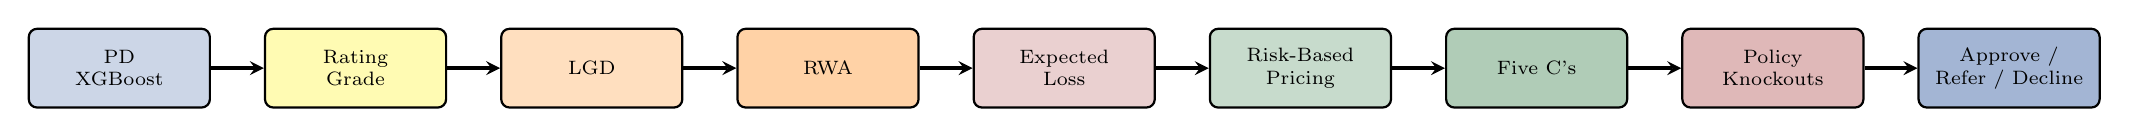
\begin{tikzpicture}[
    sbox/.style={draw, rounded corners=3pt, align=center, minimum width=2.3cm, minimum height=1.0cm,
                 inner sep=3pt, font=\scriptsize, thick},
    arr/.style={->, very thick, >=stealth}
]
\node[sbox, fill=steelblue!25]   (pd)   at (0,0)   {PD\\XGBoost};
\node[sbox, fill=yellow!30]      (rat)  at (3,0)   {Rating\\Grade};
\node[sbox, fill=orange!25]      (lgd)  at (6,0)   {LGD};
\node[sbox, fill=orange!35]      (rwa)  at (9,0)   {RWA};
\node[sbox, fill=darkred!20]     (el)   at (12,0)  {Expected\\Loss};
\node[sbox, fill=forestgreen!25] (prc)  at (15,0)  {Risk-Based\\Pricing};
\node[sbox, fill=forestgreen!35] (fc)   at (18,0)  {Five C's};
\node[sbox, fill=darkred!30]     (pol)  at (21,0)  {Policy\\Knockouts};
\node[sbox, fill=steelblue!45]   (rec)  at (24,0)  {Approve /\\Refer / Decline};
\draw[arr] (pd) -- (rat);
\draw[arr] (rat) -- (lgd);
\draw[arr] (lgd) -- (rwa);
\draw[arr] (rwa) -- (el);
\draw[arr] (el) -- (prc);
\draw[arr] (prc) -- (fc);
\draw[arr] (fc) -- (pol);
\draw[arr] (pol) -- (rec);
\end{tikzpicture}%
}
\end{center}
\vspace{8pt}
\begin{columns}[T]
  \column{0.48\textwidth}
    \begin{block}{One findings object}
      \footnotesize
      \texttt{assessment\_engine.py} produces a single JSON object with every stage above ---
      consumed by both \texttt{report-underwriter.html} (internal) and
      \texttt{report-applicant.html} (adverse-action letter).
    \end{block}
  \column{0.48\textwidth}
    \begin{block}{Explainability}
      \footnotesize
      \texttt{shap\_explainer.py} attaches SHAP-based feature attribution and counterfactual
      recourse --- \emph{``what would need to change for this applicant to qualify.''}
    \end{block}
\end{columns}
\end{frame}

% SLIDE — MASTERSCALE
\begin{frame}{Internal Rating Masterscale: PD $\to$ Grade}
\vspace{-2pt}
{\footnotesize PD is converted into a 10-grade internal scale aligned to Standardised-Approach
external rating equivalents --- consistent scoring language across ML output and regulatory reporting.}\\[6pt]
\begin{center}
\footnotesize
\begin{tabular}{lllll}
  \toprule
  \textbf{Grade} & \textbf{PD Band} & \textbf{Label} & \textbf{Inv.\ Grade} & \textbf{Decision}\\
  \midrule
  AAA & 0.00\% -- 0.50\%   & Exceptional        & Yes & \textcolor{forestgreen}{\textbf{APPROVE}}\\
  AA  & 0.50\% -- 1.00\%   & Very Strong        & Yes & \textcolor{forestgreen}{\textbf{APPROVE}}\\
  A   & 1.00\% -- 2.00\%   & Strong             & Yes & \textcolor{forestgreen}{\textbf{APPROVE}}\\
  BBB & 2.00\% -- 4.00\%   & Adequate           & Yes & \textcolor{forestgreen}{\textbf{APPROVE}}\\
  BB  & 4.00\% -- 7.00\%   & Speculative        & No  & \textcolor{amberc}{\textbf{REFER}}\\
  B   & 7.00\% -- 12.00\%  & Vulnerable         & No  & \textcolor{amberc}{\textbf{REFER}}\\
  CCC & 12.00\% -- 20.00\% & Distressed         & No  & \textcolor{darkred}{\textbf{DECLINE}}\\
  CC  & 20.00\% -- 35.00\% & Highly Distressed  & No  & \textcolor{darkred}{\textbf{DECLINE}}\\
  C   & 35.00\% -- 50.00\% & Near Default       & No  & \textcolor{darkred}{\textbf{DECLINE}}\\
  D   & 50.00\% -- 100\%   & Default            & No  & \textcolor{darkred}{\textbf{DECLINE}}\\
  \bottomrule
\end{tabular}
\end{center}
\end{frame}

% SLIDE — POLICY ENGINE
\begin{frame}{Deterministic Credit Policy --- Independent of the Model}
\vspace{-2pt}
\begin{block}{Why a separate policy engine?}
  \footnotesize
  The model produces a \textbf{risk estimate}; \texttt{policy\_engine.py} applies the bank's
  \textbf{eligibility rules and risk-appetite cutoffs}. A decline can be proven to a regulator
  as policy-driven, not a black box --- and policy can be re-versioned (\texttt{credit-policy-v1.0})
  without ever retraining the model.
\end{block}
\vspace{5pt}
\begin{center}
\footnotesize
\begin{tabular}{lll}
  \toprule
  \textbf{Rule} & \textbf{Threshold} & \textbf{Outcome}\\
  \midrule
  Sanctions / AML hit         & any match                      & \textbf{DECLINE} (hard gate)\\
  KYC incomplete              & status $\neq$ Verified          & \textbf{DECLINE}\\
  PEP flag                    & --                              & \textbf{REFER} + Enhanced DD\\
  FOIR (debt-service)         & $\geq$45\% refer / $\geq$55\% decline & REFER / DECLINE\\
  Minimum income by product   & Home Rs.\,5L, Business Rs.\,6L, Personal Rs.\,3L & REFER if below\\
  LTV cap (secured products)  & Home 80\% / Vehicle 85\% / Business 70\% & REFER if breached\\
  Age                         & $<$21 decline, maturity age $>$70 refer & DECLINE / REFER\\
  Single-borrower exposure cap & Rs.\,2\,crore                      & REFER + committee flag\\
  \bottomrule
\end{tabular}
\end{center}
\end{frame}

% SLIDE — PRICING
\begin{frame}{Risk-Based Pricing}
\vspace{-2pt}
\begin{center}
\large\textbf{Indicative Rate = Base Rate + EL Spread + Capital Charge + Operating Margin}
\end{center}
\vspace{8pt}
\begin{columns}[T]
  \column{0.48\textwidth}
    \footnotesize
    \begin{tabular}{ll}
      \toprule
      \textbf{Component} & \textbf{Default}\\
      \midrule
      Base rate (RBI repo)  & 6.50\%\\
      Min.\ capital ratio   & 8\% (Basel III Pillar 1)\\
      Target ROE            & 15\%\\
      Operating margin      & 150 bps\\
      Floor / Ceiling        & 7.0\% / 24.0\%\\
      \bottomrule
    \end{tabular}
  \column{0.48\textwidth}
    \begin{itemize}\setlength\itemsep{4pt}
      \footnotesize
      \item[\small$\bullet$] \textbf{EL Spread} = PD $\times$ LGD, expressed in bps --- the
            minimum margin to break even on expected credit losses
      \item[\small$\bullet$] \textbf{Capital Charge} = (RWA $\times$ 8\%) $\times$ target ROE,
            expressed as bps over EAD --- cost of holding regulatory capital
      \item[\small$\bullet$] Rate above the 24\% ceiling is flagged \textbf{``unviable''} ---
            the platform will not silently over-price a bad risk
    \end{itemize}
\end{columns}
\end{frame}

% ===========================================================
\section{Decision Support \& RM Workflow}
% ===========================================================

% SLIDE — MACHINE RECOMMENDATION / DOA
\begin{frame}{Machine Recommendation \& Delegation of Authority}
\vspace{-2pt}
{\footnotesize \texttt{decision\_orchestrator.py} composes model findings + policy +
confidence/OOD routing + knife-edge sensitivity into a single \textbf{Machine Recommendation (M)}
--- then decides who is authorised to act on it.}\\[6pt]
\begin{center}
\footnotesize
\begin{tabular}{lp{6.0cm}p{4.4cm}}
  \toprule
  \textbf{Control Level} & \textbf{Trigger} & \textbf{Meaning}\\
  \midrule
  \texttt{RM\_SINGLE}   & Exposure $\leq$ Rs.\,20L, high confidence & RM may finalise alone\\
  \texttt{FOUR\_EYES}   & Exposure $>$ Rs.\,20L, or LOW confidence, or knife-edge PD, or REFER & Requires credit-officer approval\\
  \texttt{COMMITTEE}    & Exposure $>$ Rs.\,1\,crore, or committee policy flag & Risk Committee only\\
  \texttt{AUTO\_DECLINE} & Hard decline / financial-crime escalation & RM cannot approve\\
  \bottomrule
\end{tabular}
\end{center}
\vspace{6pt}
\begin{alertblock}{Knife-edge detection}
  \footnotesize
  If the point-estimate PD sits within $\pm$20\% of a decision cutoff (REFER at 12\%, DECLINE at
  50\%), the recommendation is flagged \textbf{sensitive} --- a small input change could flip the
  outcome --- forcing four-eyes review even when the exposure alone would allow RM-single authority.
\end{alertblock}
\end{frame}

% SLIDE — RM WORKFLOW
\begin{frame}{Relationship Management: Machine / Human / Org Decision}
\vspace{-2pt}
\begin{columns}[T]
  \column{0.5\textwidth}
    \begin{center}
    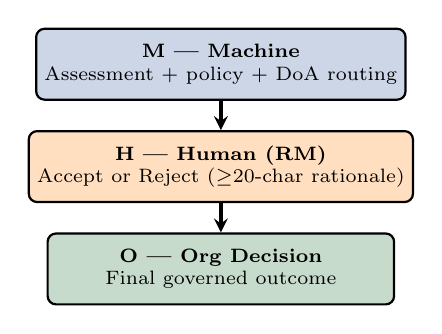
\begin{tikzpicture}[
        sbox/.style={draw, rounded corners=3pt, align=center, minimum width=4.4cm, minimum height=0.9cm,
                     inner sep=3pt, font=\scriptsize, thick},
        arr/.style={->, very thick, >=stealth}
    ]
    \node[sbox, fill=steelblue!25] (m) at (0,0)   {\textbf{M --- Machine}\\Assessment + policy + DoA routing};
    \node[sbox, fill=orange!25]    (h) at (0,-1.3) {\textbf{H --- Human (RM)}\\Accept or Reject ($\geq$20-char rationale)};
    \node[sbox, fill=forestgreen!25](o) at (0,-2.6) {\textbf{O --- Org Decision}\\Final governed outcome};
    \draw[arr] (m) -- (h);
    \draw[arr] (h) -- (o);
    \end{tikzpicture}
    \end{center}
  \column{0.46\textwidth}
    \footnotesize
    \begin{itemize}\setlength\itemsep{4pt}
      \item[\small$\bullet$] RM has \textbf{two actions only} --- accept or reject; both finalise
            immediately (no partial states)
      \item[\small$\bullet$] Every event is written to a \textbf{hash-chained} \texttt{rm\_case\_events}
            table --- tamper-evident provenance from M to O
      \item[\small$\bullet$] Outcomes feed \texttt{rm\_outcomes} for HITL (human-in-the-loop)
            learning via \texttt{/relationship/api/insights}
      \item[\small$\bullet$] \textbf{Single origination channel} --- data is captured once on the
            calculator's borrower form; the RM's ``+ New Customer'' simply navigates back to it
    \end{itemize}
\end{columns}
\end{frame}

% SLIDE — CASE LIFECYCLE / API SEQUENCE
\begin{frame}{Case Lifecycle: Onboarding to Signed-Off Report}
\vspace{-2pt}
\begin{center}
\footnotesize
\setlength{\tabcolsep}{3pt}
\begin{tabular}{*{5}{p{2.3cm}}}
  \toprule
  \cellcolor{steelblue!25}\textbf{1. Assess} &
  \cellcolor{yellow!30}\textbf{2. Refer to RM} &
  \cellcolor{orange!30}\textbf{3. RM Decision} &
  \cellcolor{forestgreen!30}\textbf{4. Generate Report} &
  \cellcolor{darkred!20}\textbf{5. Deliver PDF}\\
  \midrule
  \scriptsize\texttt{POST /api/assess-borrower} &
  \scriptsize\texttt{POST /relationship/api/cases} &
  \scriptsize\texttt{POST .../cases/id/action} &
  \scriptsize\texttt{POST .../cases/id/report} &
  \scriptsize\texttt{GET .../reports/id/ver/pdf}\\
  \bottomrule
\end{tabular}
\end{center}
\vspace{4pt}
{\footnotesize\centering $\to$ each step hands off to the next; the case is never re-entered at an earlier stage.\par}
\vspace{6pt}
\begin{columns}[T]
  \column{0.48\textwidth}
    \begin{block}{Underwriter report --- 6 sections}
      \footnotesize
      1 Risk Assessment $\cdot$ 2 Five C's Credit Assessment (2b Macro Regime Score)
      $\cdot$ 3 Peer Comparison $\cdot$ 4 Improvement Pathways $\cdot$ 5 AIRB Regulatory
      Details $\cdot$ 6 Credit Decision.
    \end{block}
  \column{0.48\textwidth}
    \begin{block}{PDF generation \& versioning}
      \footnotesize
      \texttt{report\_generator.py}: matplotlib charts $\to$ LaTeX $\to$ pdflatex. Every
      report is versioned under \texttt{data/case\_reports/<case\_id>/<version>/} --- regenerating
      a report never overwrites a prior version.
    \end{block}
\end{columns}
\end{frame}

% ===========================================================
\section{Operations, Regulatory \& Financial Reporting}
% ===========================================================

% SLIDE — OPERATIONS
\begin{frame}{Banking Operations \& Regulatory Reporting}
\vspace{-2pt}
\begin{columns}[T]
  \column{0.48\textwidth}
    \begin{block}{Banking Operations (\texttt{/operations/})}
      \footnotesize
      \begin{itemize}\setlength\itemsep{3pt}
        \item[\small$\bullet$] Multi-bank dashboard --- 9 banks, live customer/account/loan ledger
        \item[\small$\bullet$] Loan portfolio by status (Active, NPA, Defaulted, Written-Off, Closed)
        \item[\small$\bullet$] Per-customer 360$^\circ$ view: accounts, loans, transactions
        \item[\small$\bullet$] NPA resolution workflow; live DB schema viewer for admins
      \end{itemize}
    \end{block}
  \column{0.48\textwidth}
    \begin{block}{Regulatory Reporting (\texttt{/regulatory/})}
      \footnotesize
      \begin{itemize}\setlength\itemsep{3pt}
        \item[\small$\bullet$] Basel III / RBI: CRAR $\geq$11.5\%, Tier-1 $\geq$9.5\%, CET1 $\geq$8\%
        \item[\small$\bullet$] Liquidity: LCR $\geq$100\%, NSFR $\geq$100\%, CRR $\geq$4.5\%, SLR $\geq$18\%
        \item[\small$\bullet$] Per-client RWA exposures rolled up to bank-level capital reports
        \item[\small$\bullet$] Daily batch (APScheduler, 01:00) + on-demand \texttt{run-batch}
      \end{itemize}
    \end{block}
\end{columns}
\vspace{6pt}
\begin{alertblock}{Same ledger, no reconciliation}
  \footnotesize
  Both departments read the \emph{same} \texttt{bank.db} loan/account records that the Credit Risk
  calculator writes to --- capital ratios and NPA figures are always consistent with the
  underlying originated exposures.
\end{alertblock}
\end{frame}

% SLIDE — FINANCIALS + REFERENCE
\begin{frame}{Financial Reporting \& Global Reference Data}
\vspace{-2pt}
\begin{columns}[T]
  \column{0.48\textwidth}
    \begin{block}{Financial Reporting (\texttt{/financials/})}
      \footnotesize
      \begin{itemize}\setlength\itemsep{3pt}
        \item[\small$\bullet$] Balance Sheet, P\&L, Key Ratios, Pillar 3 disclosures
        \item[\small$\bullet$] One generic \texttt{consolidate()} function produces bank / region /
              country / group roll-ups from the same code path
        \item[\small$\bullet$] Versioned PDF annual reports per scope
        \item[\small$\bullet$] Foreign banks use a 75\% average risk weight where loan-level detail
              is unavailable
      \end{itemize}
    \end{block}
  \column{0.48\textwidth}
    \begin{block}{Global Reference Data (\texttt{/reference/})}
      \footnotesize
      \begin{itemize}\setlength\itemsep{3pt}
        \item[\small$\bullet$] \texttt{countries} --- ISO-3, region, Basel minimums, sovereign rating
        \item[\small$\bullet$] \texttt{country\_macro} --- GDP, CPI, policy rate, FX (2 periods/country)
        \item[\small$\bullet$] 7 countries seeded; feeds the ML model's macro features and the
              onboarding form's country selector
      \end{itemize}
    \end{block}
\end{columns}
\vspace{8pt}
\begin{block}{Global hierarchy}
  \footnotesize
  Group $\to$ Region $\to$ Country $\to$ Bank. 9 real-world banks grounded in FY2025 annual
  reports --- India (HDFC, ICICI, Bank of Baroda, PNB), USA (JPMorgan Chase), UK (Barclays),
  Singapore (DBS), UAE (Emirates NBD), Australia (Commonwealth Bank) --- all foreign ledgers
  denominated in group reporting currency (Rs.\,).
\end{block}
\end{frame}

% ===========================================================
\section{End-to-End Use Cases by Exposure Segment}
% ===========================================================

% SLIDE — SEGMENT MAP
\begin{frame}{Four Exposure Segments, One Onboarding Form}
\vspace{-2pt}
{\footnotesize The same \texttt{borrower-info.html} intake form serves every customer type ---
an \textbf{Exposure Class} dropdown routes the application to the matching PD model, risk weight,
and downstream policy checks. The next four slides walk each segment end-to-end.}\\[8pt]
\begin{center}
\footnotesize
\begin{tabular}{lp{2.9cm}rrp{4.0cm}}
  \toprule
  \textbf{Exposure Class} & \textbf{Typical Customer} & \textbf{SA RW} & \textbf{PD AUC} & \textbf{Key Inputs}\\
  \midrule
  CORPORATE          & Large corporate borrower   & 100\% & 0.754 & DE ratio, interest coverage, profitability\\
  SME                & Small/medium enterprise    & 85\%  & 0.764 & Liquidity ratio, turnover, collateral\\
  RETAIL\_MORTGAGES  & Home loan applicant        & 35\%  & 0.758 & Income, LTV, CIBIL, employment\\
  RETAIL\_OTHER      & Personal/vehicle/education & 75\%  & 0.753 & FOIR, CIBIL, dependents, tenure\\
  \bottomrule
\end{tabular}
\end{center}
\vspace{8pt}
\begin{block}{Common intake fields (all segments)}
  \footnotesize
  Borrower ID/Name, Exposure Amount, Country, KYC status, sanctions screening, proposed EMI,
  existing obligations, sector, loan type (auto-sets maturity), collateral type/value,
  seniority, LTV. Retail applications add age, employment, CIBIL score, FOIR, dependents; Corporate/SME
  applications add the four financial ratios that feed the model directly.
\end{block}
\end{frame}

% SLIDE — USE CASE 1: CORPORATE
\begin{frame}{Use Case 1 --- CORPORATE: Large Working-Capital Facility}
\vspace{-2pt}
\begin{columns}[T]
  \column{0.55\textwidth}
    \footnotesize
    \textbf{Scenario:} A mid-size manufacturer requests a Rs.\,15\,crore working-capital facility.
    \begin{enumerate}\setlength\itemsep{4pt}
      \item[\textbf{1.}] \textbf{Onboard} --- RM enters borrower financials: DE ratio, interest
            coverage, profitability margin, liquidity ratio; Exposure Class = \texttt{CORPORATE}
      \item[\textbf{2.}] \textbf{Score} --- CORPORATE XGBoost model returns PD; masterscale maps
            it to a grade (e.g.\ BBB, 3.1\% PD $\to$ APPROVE band)
      \item[\textbf{3.}] \textbf{Policy} --- single-borrower cap (Rs.\,2\,crore) is exceeded by the
            requested Rs.\,15\,crore $\to$ \texttt{SINGLE\_BORROWER\_CAP} fires, \texttt{COMMITTEE\_REQUIRED} flag set
      \item[\textbf{4.}] \textbf{Route} --- exposure $>$ Rs.\,1\,crore $\to$ \texttt{COMMITTEE} control level;
            RM cannot finalise alone
      \item[\textbf{5.}] \textbf{Decide \& Report} --- Risk Committee reviews the Machine
            Recommendation, accepts with conditions; underwriter PDF generated and versioned
    \end{enumerate}
  \column{0.42\textwidth}
    \begin{block}{Why this matters}
      \footnotesize
      Large corporate exposures automatically escalate past RM authority --- the platform
      enforces committee governance \emph{before} any human has a chance to approve outside policy.
    \end{block}
    \vspace{5pt}
    \begin{block}{Output}
      \footnotesize
      Rating grade, RWA/EL/capital charge, indicative pricing, Five C's narrative, committee-ready
      PDF with full audit trail.
    \end{block}
\end{columns}
\end{frame}

% SLIDE — USE CASE 2: SME
\begin{frame}{Use Case 2 --- SME: Business Expansion Loan}
\vspace{-2pt}
\begin{columns}[T]
  \column{0.55\textwidth}
    \footnotesize
    \textbf{Scenario:} A retail-chain SME requests a Rs.\,35\,lakh business loan against
    Rs.\,50\,lakh collateral.
    \begin{enumerate}\setlength\itemsep{4pt}
      \item[\textbf{1.}] \textbf{Onboard} --- Exposure Class = \texttt{SME}; LTV = 35L/50L = 70\%
            (exactly at the Business Loan policy cap of 70\%)
      \item[\textbf{2.}] \textbf{Score} --- SME model (AUC 0.764) returns PD; grade BB $\to$ REFER band
      \item[\textbf{3.}] \textbf{Policy} --- LTV at the boundary passes; minimum-income gate for
            Business Loan (Rs.\,6L) is checked against the SME's declared income
      \item[\textbf{4.}] \textbf{Route} --- BB grade + REFER model output $\to$ \texttt{FOUR\_EYES}
            control level even though exposure (Rs.\,35L) is above the Rs.\,20L RM-single ceiling anyway
      \item[\textbf{5.}] \textbf{Decide \& Report} --- Credit officer reviews SHAP attribution
            and counterfactual recourse (``what would move this to APPROVE''), accepts with
            conditions (reduce quantum or add collateral)
    \end{enumerate}
  \column{0.42\textwidth}
    \begin{block}{Why this matters}
      \footnotesize
      SME risk sits in the volatile middle band --- the platform's knife-edge sensitivity check
      is exactly the safeguard this segment needs.
    \end{block}
    \vspace{5pt}
    \begin{block}{Output}
      \footnotesize
      Conditional approval with explicit remediation levers, indicative rate reflecting the
      85\% SA risk weight, applicant-facing adverse-action letter if declined.
    \end{block}
\end{columns}
\end{frame}

% SLIDE — USE CASE 3: RETAIL_MORTGAGES
\begin{frame}{Use Case 3 --- RETAIL\_MORTGAGES: Home Loan}
\vspace{-2pt}
\begin{columns}[T]
  \column{0.55\textwidth}
    \footnotesize
    \textbf{Scenario:} A salaried individual, age 34, requests a Rs.\,45\,lakh home loan against a
    Rs.\,60\,lakh property.
    \begin{enumerate}\setlength\itemsep{4pt}
      \item[\textbf{1.}] \textbf{Onboard} --- Exposure Class = \texttt{RETAIL\_MORTGAGES};
            LTV = 45L/60L = 75\% (within the 80\% Home Loan cap); CIBIL, FOIR, employment
            tenure captured
      \item[\textbf{2.}] \textbf{Score} --- RETAIL\_MORTGAGES model (AUC 0.758) returns PD; grade
            A $\to$ APPROVE band
      \item[\textbf{3.}] \textbf{Policy} --- income Rs.\,8L $>$ Rs.\,5L Home Loan minimum, age 34 with
            20-year tenor $\to$ maturity age 54 $<$ 70 cap --- all rules clear
      \item[\textbf{4.}] \textbf{Route} --- exposure Rs.\,45L $>$ Rs.\,20L RM-single ceiling
            $\to$ \texttt{FOUR\_EYES}, but high confidence and no knife-edge means fast-track review
      \item[\textbf{5.}] \textbf{Decide \& Report} --- Credit officer accepts; borrower receives
            a plain-language applicant letter with indicative rate at the 35\% mortgage risk weight
    \end{enumerate}
  \column{0.42\textwidth}
    \begin{block}{Why this matters}
      \footnotesize
      Mortgages carry the lowest SA risk weight (35\%) --- pricing and capital charge are
      materially lower than an equivalent unsecured personal loan, visible directly in the
      pricing breakdown.
    \end{block}
\end{columns}
\end{frame}

% SLIDE — USE CASE 4: RETAIL_OTHER
\begin{frame}{Use Case 4 --- RETAIL\_OTHER: Personal Loan (Declined, then Recourse)}
\vspace{-2pt}
\begin{columns}[T]
  \column{0.55\textwidth}
    \footnotesize
    \textbf{Scenario:} An applicant with FOIR 58\% requests a Rs.\,4\,lakh personal loan.
    \begin{enumerate}\setlength\itemsep{4pt}
      \item[\textbf{1.}] \textbf{Onboard} --- Exposure Class = \texttt{RETAIL\_OTHER};
            FOIR computed from existing obligations + proposed EMI over monthly income
      \item[\textbf{2.}] \textbf{Score} --- RETAIL\_OTHER model (AUC 0.753) returns PD;
            independently, FOIR 58\% $\geq$ 55\% \texttt{FOIR\_EXCEEDS\_LIMIT} $\to$ \textbf{DECLINE}
      \item[\textbf{3.}] \textbf{Policy dominates} --- \texttt{\_compose()} takes the
            \emph{worst of} model and policy; a policy DECLINE overrides even a favourable model grade
      \item[\textbf{4.}] \textbf{Route} --- \texttt{AUTO\_DECLINE} --- RM cannot approve, escalation only
      \item[\textbf{5.}] \textbf{Recourse} --- counterfactual engine returns actionable levers
            (e.g.\ ``reduce requested EMI by Rs.\,X to bring FOIR under 55\%''); applicant-facing
            adverse-action letter cites the specific reason code, not a black-box score
    \end{enumerate}
  \column{0.42\textwidth}
    \begin{block}{Why this matters}
      \footnotesize
      Demonstrates that \textbf{policy always wins} over the model when they disagree --- and that
      every decline ships with a specific, actionable, regulator-defensible reason.
    \end{block}
\end{columns}
\end{frame}

% ===========================================================
\section{Governance \& Roadmap}
% ===========================================================

% SLIDE — GOVERNANCE
\begin{frame}{Governance, Auditability \& Explainability}
\vspace{-2pt}
\begin{columns}[T]
  \column{0.48\textwidth}
    \begin{block}{Traceability}
      \footnotesize
      \begin{itemize}\setlength\itemsep{3pt}
        \item[\small$\bullet$] Hash-chained \texttt{rm\_case\_events} --- every M/H/O step is
              content-hashed and linked to the previous event
        \item[\small$\bullet$] \texttt{content\_hash} on the Machine Recommendation itself ---
              tamper-evident, reproducible from inputs
        \item[\small$\bullet$] Model version, policy version (\texttt{credit-policy-v1.0}), and
              report ID all stamped on every decision
      \end{itemize}
    \end{block}
  \column{0.48\textwidth}
    \begin{block}{Explainability}
      \footnotesize
      \begin{itemize}\setlength\itemsep{3pt}
        \item[\small$\bullet$] SHAP-based per-feature attribution on every score
        \item[\small$\bullet$] Counterfactual recourse --- specific, actionable levers for declined
              or borderline applicants
        \item[\small$\bullet$] Peer benchmarking --- segment-scoped comparison against approved
              borrowers in the same exposure class
      \end{itemize}
    \end{block}
\end{columns}
\vspace{8pt}
\begin{alertblock}{Model does not decide alone}
  \footnotesize
  The ML model estimates risk; \texttt{policy\_engine.py} enforces eligibility; \texttt{decision\_orchestrator.py}
  determines who may act; a human RM or committee makes the final call. No exposure is
  auto-approved by the model in isolation.
\end{alertblock}
\end{frame}

% SLIDE — ROADMAP
\begin{frame}{Recent Progress \& Roadmap}
\vspace{-2pt}
\begin{columns}[T]
  \column{0.48\textwidth}
    \textbf{Recent phases}
    \begin{itemize}\setlength\itemsep{4pt}
      \footnotesize
      \item[\small$\bullet$] Real transaction-derived behavioural features (EMI-miss ratio,
            income volatility)
      \item[\small$\bullet$] 5-fold CV AUC alongside single-split AUC in the training pipeline
      \item[\small$\bullet$] ALM engine, loan booking \& NPA resolution workflow added
      \item[\small$\bullet$] PD models split by Basel exposure class --- retired the single
            unsegmented model
      \item[\small$\bullet$] SHAP-based explainability layer integrated into assessment output
    \end{itemize}
  \column{0.48\textwidth}
    \textbf{Roadmap}
    \begin{itemize}\setlength\itemsep{4pt}
      \footnotesize
      \item[\small$\bullet$] \textbf{Phase 6} --- GCP App Engine deployment (in progress)
      \item[\small$\bullet$] \textbf{Phase 7} --- Operational Risk (TSA / AMA)
      \item[\small$\bullet$] \textbf{Phase 8} --- Market Risk (VaR)
    \end{itemize}
\end{columns}
\end{frame}

% SLIDE — THANK YOU
\begin{frame}
  \begin{center}
    \vspace{1.0cm}
    {\Large\bfseries Thank You}\\[8pt]
    {\normalsize Questions \& Discussion}

    \vspace{0.8cm}
    \footnotesize
    \begin{tabular}{rl}
      \textbf{Solution:}  & Banking Credit Risk Calculator\\
      \textbf{Coverage:}  & Credit Risk $\cdot$ Operations $\cdot$ Regulatory $\cdot$ RM $\cdot$ Financials $\cdot$ Reference Data\\
      \textbf{Deployment:} & GCP App Engine\\
    \end{tabular}

    \vspace{0.7cm}
    \small\textit{Basel III Compliant, ML-Powered Credit Risk Platform}
  \end{center}
\end{frame}

\end{document}
